\documentclass{beamer}
\usetheme{Copenhagen}


\title{Tutorial VS Code, bash y github}
\author{\texorpdfstring{Author\newline\url{www.github.com/mlacosta}}{Author}}
\author{Ing. Mariano L. Acosta}
\logo{
\includegraphics[width=.1\textwidth]{img/logo.jpg}}

\begin{document}
\begin{frame}[plain]
    \maketitle
\end{frame}


\begin{frame}
	\frametitle{Contenidos}
	\tableofcontents
\end{frame}

\section{Presentación de Herramientas}

\begin{frame}{Virtual Studio Code}
	\begin{columns}
  		\begin{column}{.5\textwidth}
			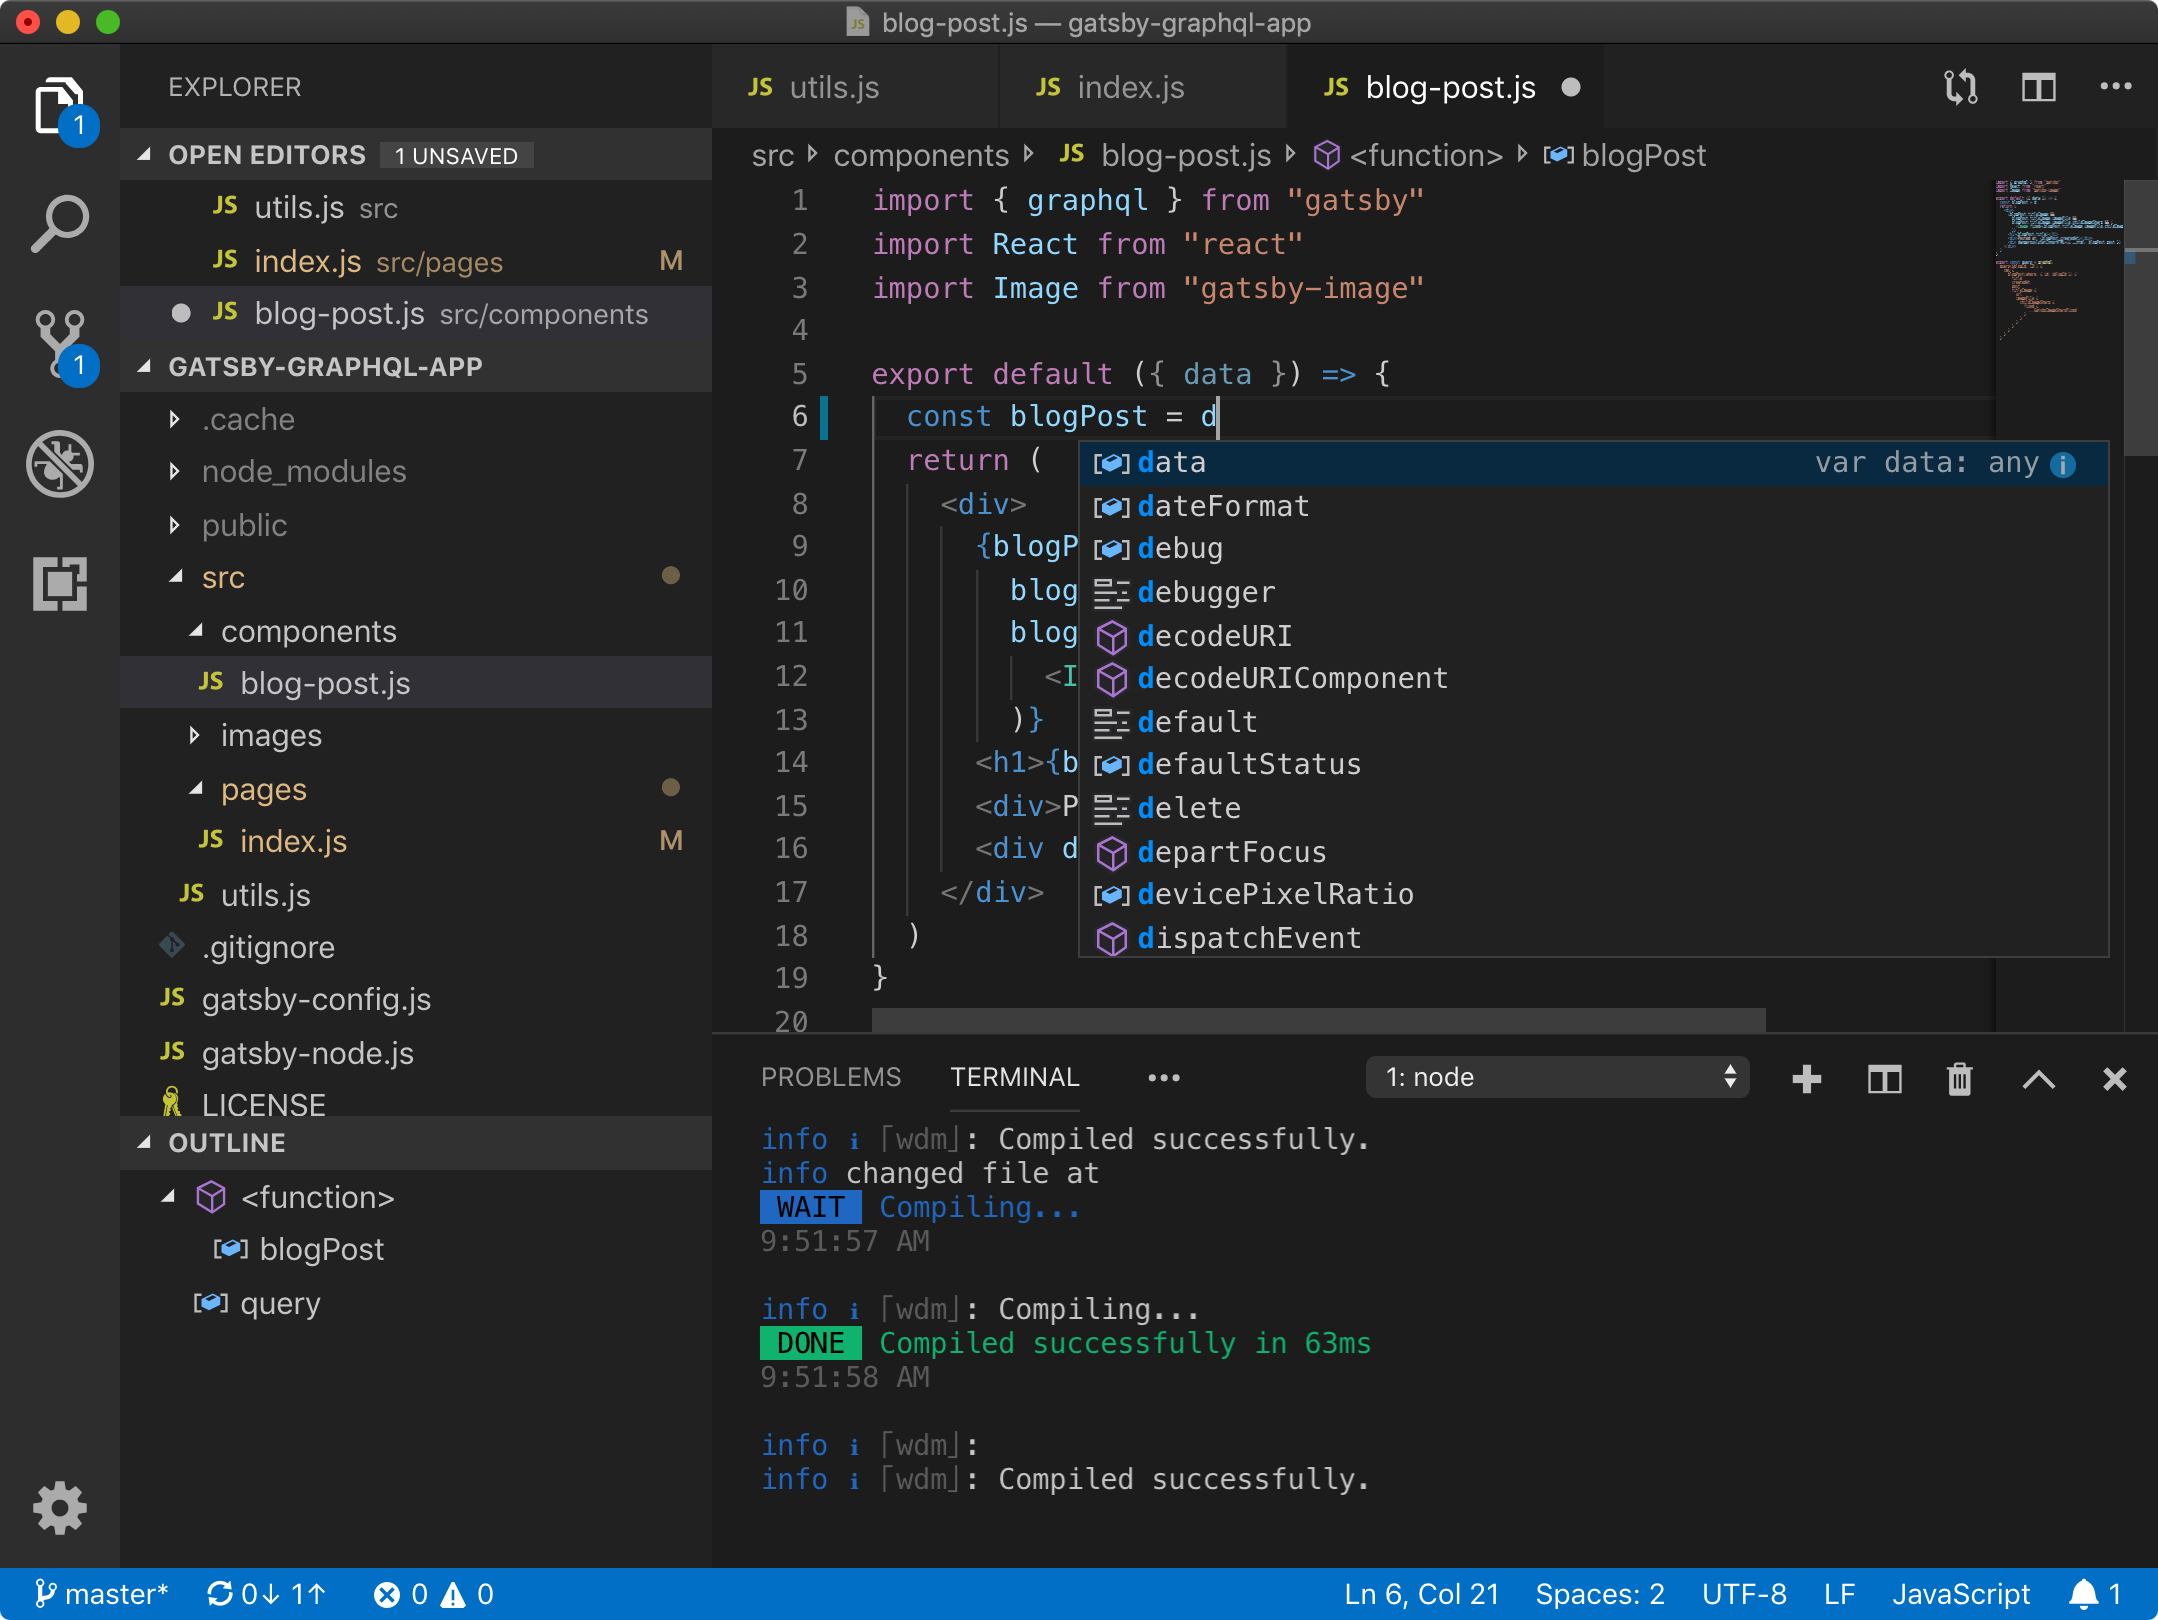
\includegraphics[scale=.15]{img/vscode.png}
		\end{column}
		\begin{column}{.5\textwidth}
				
			\begin{itemize}
				\item IntelliSense (autocompletado de código, info extra, etc.)
				\item Altamente customizable (plugins/temas)
				\item Prestaciones optimizadas para desarrollo web
				\item Integración con JSX/React, HTML, CSS, JSON, etc...
			\end{itemize}
		\end{column}
	\end{columns}
\end{frame}

\begin{frame}{Bash Shell (Windows)}
	\begin{columns}
		\begin{column}{.5\textwidth}
			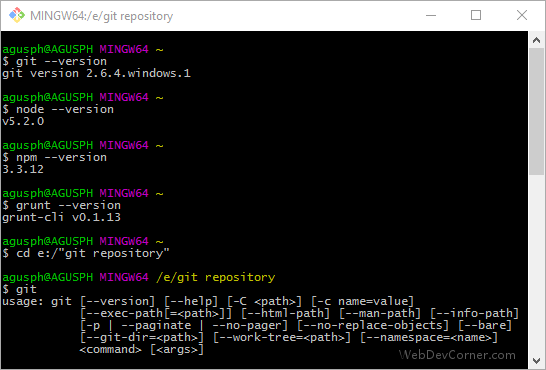
\includegraphics[scale=.3]{img/git_bash.png}
		\end{column}
		\begin{column}{.5\textwidth}
			
			\begin{itemize}
				\item Emulación de la linea de comandos de UNIX
				\item Amigable para principiantes y expertos
				\item Automatización de tareas repetitivas (scripts)
				\item Soporte de la comunidad (recursos disponibles)
			\end{itemize}
		\end{column}
	\end{columns}
	
\end{frame}

\begin{frame}{Git | Control de Versiones}
	\begin{columns}
		\begin{column}{.3\textwidth}
			
\includegraphics[scale=.1]{img/git_logo.png}
		\end{column}
		\begin{column}{.6\textwidth}
			
			\begin{itemize}
				\item Registros de todos los cambios en el código (undoing)
				\item Colaboración con múltiples desarrolladores (branching)
				\item Prototipado/Desarrollo de prestaciones (features)
			\end{itemize}
		\end{column}
	\end{columns}
\end{frame}

\begin{frame}{Git | Control de Versiones}

	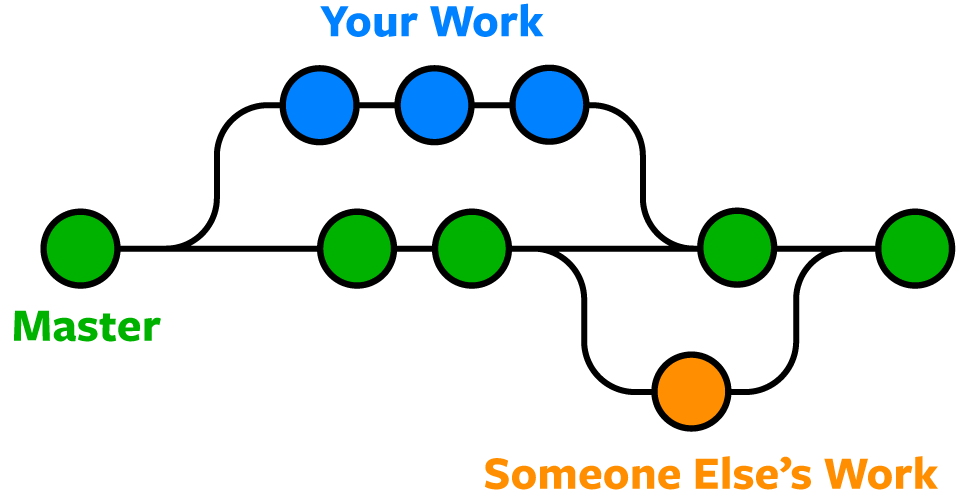
\includegraphics[scale=.3]{img/branches.png}
	
\end{frame}

\begin{frame}{Git | Control de Versiones}
	
	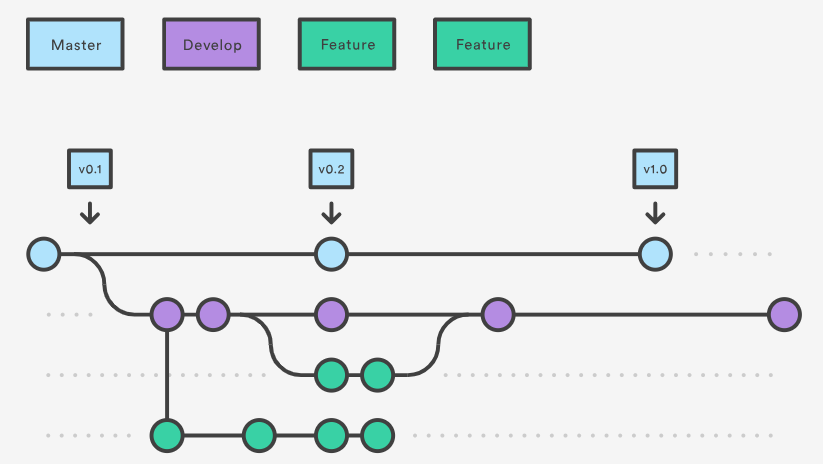
\includegraphics[scale=.35]{img/git_project.png}
	
\end{frame}

\begin{frame}{Github}
	\begin{columns}
		\begin{column}{.45\textwidth}
			
\includegraphics[scale=.12]{img/github.jpeg}
		\end{column}
		\begin{column}{.55\textwidth}
			
			\begin{itemize}
				\item Emulación de la linea de comandos de UNIX
				\item Amigable para principiantes y expertos
				\item Automatización de tareas repetitivas (scripts)
				\item Soporte de la comunidad (recursos disponibles)
			\end{itemize}
		\end{column}
	\end{columns}
	
\end{frame}


\section{Comandos de Consola (Bash)}

\section{Comandos de Git}

\end{document}
